\documentclass[../main.tex]{subfiles}
\begin{document}
\chapter{Vector Differential Operators}
An operator is a map between vector spaces.
\section{Del}
\begin{definition}
  The fundamental differential operator is \textit{del}:
  \[
    \nabla = \begin{pmatrix}
    \partial/\partial x_1 \\
    \partial/\partial x_2 \\
    \partial/\partial x_3 \\
    \end{pmatrix}
  \]
\end{definition}
This operator is applied in various ways to scalar and vector fields as we will see throughout this chapter.
In this context, a \textit{field} is simply a quantity that depends on $\vec{x}$.
\begin{remark}
  Del is often called ``grad'' although this is not strictly correct as grad is a specific operator derived from del.
\end{remark}
We can also write:
\[
  \nabla = \vec{e}_1 \pderiv{}{x} + \vec{e}_2 \pderiv{}{y} + \vec{e}_3 \pderiv{}{z} = \vec{e}_i \pderiv{}{x_i}
\]
where $\{\vec{e}_1, \vec{e}_2, \vec{e}_3\}$ is the standard basis for $\R^{3}$.
\section{Gradient}
\label{secGrad}
\begin{definition}[Gradient]
  When del is applied to a \textbf{scalar field} $f(\vec{x})$, it is known as the \textit{gradient operator}:
  \[
    \nabla f = \begin{pmatrix}
    \partial f/\partial x \\
    \partial f/\partial y \\
    \partial f/\partial z \\
    \end{pmatrix}
  \]
  or in suffix notation:
  \[
    (\nabla f)_i = \pderiv{f}{x_i},\ \nabla f = \pderiv{f}{x_i}\vec{e}_i
  \]
\end{definition}
\begin{example}[Using Grad]
  \label{gradExample}
  \begin{enumerate}
    \item If $f(\vec{x}) = |\vec{x}| = x^2 + y^2 + z^2$, then $\nabla f = (2x, 2y, 2z) = 2\vec{x}$.

      Alternatively, we can use suffix notation and summation convention:
      \[
        \pderiv{}{x_i}(x_j x_j) = 2x_j \pderiv{x_j}{x_i} = 2x_j \delta_{i j} = 2x_i
      \]
    \item $\nabla |\vec{x} - \vec{x}_0|^2 = 2(\vec{x} - \vec{x}_0)$.
      We can evaluate this component wise, or use suffix notation and summation convention like above.
      However, if we shift the origin by letting $\vec{x}' = \vec{x} - \vec{x}_0$, then using multivariate chain rule \cref{MVC}:
      \[
      \pderiv{}{x_i'} = \pderiv{x_j}{x_i'} \pderiv{}{x_j} = \pderiv{}{x_i'}(x'_j + {x_0}_j) \pderiv{}{x_j} = \delta_{i j} \pderiv{}{x_j} = \pderiv{}{x_i}
      \]
      so $\nabla_{\vec{x}} |\vec{x} - \vec{x}_0|^2 = \nabla_{\vec{x}'} |\vec{x}'| = 2\vec{x}' = 2(\vec{x} - \vec{x}_0)$.
    \item For constant $\vec{a}$, $\nabla(\vec{a} \cdot \vec{x}) = \nabla(a_1 x + a_2 y + a_3 z) = (a_1, a_2, a_3) = \vec{a}$.
      Alternatively, $\pderiv{ }{x_i} (a_j x_j) = a_j \delta_{i j} = a_i$.
  \end{enumerate}
\end{example}
Similarly to $f'$ in 1D, if we need to specify where $\nabla f$ is evaluated at, we write $\nabla f(\vec{x}_1)$.
\begin{example}
  If $f(\vec{x}) = x + y^2 + z^{4}$ then $\nabla f(\vec{a}) = \nabla f(\vec{b})$ if and only if $\vec{a} - \vec{b}$ is parallel to the $x$-axis.

  $\nabla f(\vec{x}) = (1, 2y, 4z^3)$ so $\nabla f(\vec{a}) = \nabla f(\vec{b}) \iff (1, 2a_2, 4a^{3}_{3}) = (1, 2b_2, 4b^{3}_{3})$, that is $a_2 = b_2$ and $b_3$, so $\vec{a} - \vec{b} = (a_1 - b_1, 0, 0) \parallel \vec{e}_1$.
\end{example}
\begin{remark}[Notation]
  $\nabla f(2\vec{x})$ means find $\nabla f$ and then evaluate it at $2\vec{x}$, whereas $\nabla (f(2\vec{x}))$ means evaluate at $2\vec{x}$ and then find $\nabla$ of that.

  It is often easier to avoid ambiguity by defining a new variable, for example, $\vec{y} = 2\vec{x}$ so $\nabla (f(2\vec{x})) = 2 \nabla f(\vec{y})$.

  Similarly, in 2D we can unambiguously write:
  \[
    \at{\pderiv{}{u} f(u, v)}{u = 2x, v = 2y}
  \]
  instead of $f_x(2x, 2y)$ where it is ambiguous whether the partial is taken before or after substituting $(2x, 2y)$.
\end{remark}
We can rewrite the multivariate chain rule using grad:
\begin{equation}
  \deriv{}{t}f(\vec{x}(t)) = \dot{\vec{x}} \cdot \nabla f \label{MVCGrad}
\end{equation}
and in terms of infinitesimals as:
\begin{equation}
  \d{f} = \nabla f \cdot \d{\vec{x}} \label{infinitesimalsGrad}
\end{equation}
This gives us an alternative way to define $\nabla f$ that is coordinate independent, that is, we do not have to choose a particular basis before using it.
Given a function $f$, we can define $\nabla f$ to be the unique vector such that satisfies the above for every possible choice of $\d{\vec{x}}$.
\begin{example}
  Suppose we want to find $\nabla f$ for $f(\vec{x}) = |\vec{x}|^2$, then:
  \begin{align*}
    \d{f} = f(x + \d{\vec{x}}) - f(\vec{x}) &= \vec{x} \cdot \vec{x} + 2\vec{x} \cdot \d{\vec{x}} + \cancelto{0}{\d{\vec{x}} \cdot \d{\vec{x}}} - |\vec{x}|^2 \\
                                            &= 2\vec{x} \cdot \d{\vec{x}}
  \end{align*}
  so $\nabla f = 2\vec{x}$ by definition which agrees with \cref{gradExample}.
\end{example}
Sometimes we wish to differentiate with respect to the components of a vector other than $\vec{x}$.
We denote this $\nabla_{\vec{y}} \equiv \vec{e}_i \pderiv{}{y_i}$.
\begin{example}
  Consider $f(\vec{x}, \vec{y}) = |\vec{x} - 2\vec{y}|^2$.
  We know from \cref{gradExample} that $\nabla |\vec{x} - \vec{x}_0|^2 = 2(\vec{x} - \vec{x}_0)$ for a constant vector $\vec{x}_0$.
  Since $\vec{y}$ is a constant vector with respect to $\vec{x}$, $\nabla f = 2(\vec{x} - 2\vec{y})$.

  However if we are taking grad with respect to $\vec{y}$, $\vec{x}$ is a constant vector so:
  \[
    \nabla_{\vec{y}} |\vec{x} - 2\vec{y}|^2 = -2 \cdot 2 (\vec{x} - 2\vec{y}) = -4(\vec{x} - 2\vec{y})
  \]
  This can also be checked using suffix notation.
\end{example}

\section{Divergence}
\label{secDiv}
\begin{definition}[Divergence]
If we take the dot product of del with a \textbf{vector field} $\vec{F}(\vec{x})$, then we get the \textit{divergence operator}:
\[
  \nabla \cdot \vec{F} = \begin{pmatrix}
    \partial/\partial x_1 \\
    \partial/\partial x_2 \\
    \partial/\partial x_3 \\
    \end{pmatrix} \cdot
    \begin{pmatrix}
    F_1 \\
    F_2 \\
    F_3 \\
    \end{pmatrix} =
    \pderiv{F_1}{x} + \pderiv{F_2}{y} + \pderiv{F_3}{z}
\]
or in suffix notation:
\[
  \nabla \cdot \vec{F} = \pderiv{F_i}{x_i}
\]
\end{definition}
To obtain the suffix notation expression we can use:
\begin{align*}
  \nabla \cdot \vec{F} &= \left(\vec{e}_i \pderiv{}{x_i}\right) \cdot (F_j \vec{e}_j) \\
                       &= \vec{e}_i \cdot \pderiv{F_j}{x_i} \vec{e}_j \\
                       &= \pderiv{F_j}{x_i} \delta_{i j} = \pderiv{F_j}{x_i}\\
\end{align*}
$\partial/\partial x_i$ is a scalar operator so can be moved ``through'' the dot product as:
\[
  \left(\vec{a} \pderiv{}{x_i}\right) \cdot \vec{b} =
  \left[\begin{pmatrix}
  a_1 \\
  a_2 \\
  a_3 \\
  \end{pmatrix} \pderiv{}{x_i}\right] \cdot \vec{b} =
  \begin{pmatrix}
  a_1 \pderiv{}{x_1} \\
  a_2 \pderiv{}{x_2} \\
  a_3 \pderiv{}{x_3} \\
  \end{pmatrix} \cdot
  \begin{pmatrix}
  b_1 \\
  b_2 \\
  b_3 \\
  \end{pmatrix}
  = \vec{a} \cdot \begin{pmatrix}
  \pderiv{b_1}{x_1} \\
  \pderiv{b_2}{x_2} \\
  \pderiv{b_3}{x_3} \\
  \end{pmatrix} =
  \vec{a} \cdot \left(\pderiv{}{x_i} \vec{b}\right)
\]
Roughly speaking, the divergence of a vector field at $\vec{x}$, measures the amount at which the field is expanding around $\vec{x}$.
Later in the course we will derive a coordinate-independent definition of $\nabla \cdot \vec{F}$.
\begin{example}[Using Divergence]
  \begin{enumerate}
    \item $F(\vec{x}) = \vec{x} = (x, y, z)$ so $\nabla \cdot \vec{F} = \pderiv{x}{x} + \pderiv{y}{y} + \pderiv{z}{z} = 3$, or using suffix notation, $F_i = x_i$ so $\nabla \cdot \vec{F} = \delta_{i i} = 3$.
      \begin{center}
      \begin{tikzpicture}[scale=1.13]
        \begin{scope}
          \clip (-2,-2) rectangle (2,2);
          \foreach \x in {-2, -1.5, ..., 2} {
              \foreach \y in {-2, -1.5, ..., 2} {
                  \draw[-{Stealth[length=3pt,width=4.6pt]}] (\x, \y) -- (\x*1.5,\y*1.5);
              }
          }
        \end{scope}
      \end{tikzpicture}
      \end{center}
      We see that the vector field is expanding so agrees with our rough interpretation of the divergence.
    \item $\vec{F}(\vec{x}) = (-y, x, 0)$ so $\nabla \cdot \vec{F} = -\pderiv{y}{x} + \pderiv{x}{y} = 0$.
    \item If $A$ is a $3 \times 3$ matrix then.
      \[
        \nabla \cdot (A \vec{x}) = \pderiv{}{x_i}(A_{i j }x_j) = A_{i j}\delta_{i j} = \tr A
      \]
      This works as we are using $\vec{F}(\vec{x}) = A\vec{x}$ so it is acting on a vector field.
      This means that the trace of a matrix loosely represents how much the vector field associated with $A$ is expanding around any point.
  \end{enumerate}
\end{example}
\section{Curl}
\label{secCurl}
\begin{definition}[Curl]
  The \textit{curl} of a \textbf{vector field} $\vec{F}(\vec{x})$ is defined as:
  \[
    \nabla \times \vec{F} = \begin{pmatrix}
      \partial/\partial x_1 \\
      \partial/\partial x_2 \\
      \partial/\partial x_3 \\
      \end{pmatrix} \times
      \begin{pmatrix}
      F_1 \\
      F_2 \\
      F_3 \\
      \end{pmatrix} =
      \begin{pmatrix}
      \pderiv{F_3}{y} - \pderiv{F_2}{z} \\
      \pderiv{F_1}{z} - \pderiv{F_3}{x} \\
      \pderiv{F_2}{x} - \pderiv{F_1}{y} \\
      \end{pmatrix}
  \]
  or in suffix notation:
  \[
    (\nabla \times \vec{F})_i = \levi_{i j k} \pderiv{}{x_j} F_k \text{ or equivalently } \nabla \times \vec{F} = \levi_{i j k} \pderiv{F_k}{x_j} \vec{e}_i
  \]
\end{definition}
\begin{remark}
  Curl is only defined in 3D due to the presence of a cross product, unlike grad and div which are defined in any dimension.
\end{remark}
We can also use the determinant form for the cross product to write:
\[
  \nabla \times \vec{F} = \begin{vmatrix}
  \vec{e}_1 & \vec{e}_2 & \vec{e}_3 \\
  \pderiv{}{x} & \pderiv{}{y} & \pderiv{}{z} \\
  F_1 & F_2 & F_3 \\
  \end{vmatrix}
\]
However, this only works if the determinant is expanded along the top row but is useful for memorisation nevertheless.

Roughly speaking, the curl of a vector field at a point $\vec{x}$ measures the rotation of the field around $\vec{x}$ although this will be explored more rigorously later.
The modulus $|\nabla \times \vec{F}|$ gives the magnitude of the rotation while its direction gives the axis.
\begin{example}[Using Curl]
  \begin{enumerate}
    \item With $\vec{F}(\vec{x}) = (x, y, z)$:
      \[
        \nabla \times \vec{F} = \begin{pmatrix}
        \pderiv{}{x} \\
        \pderiv{}{y} \\
        \pderiv{}{z} \\
        \end{pmatrix} \times \begin{pmatrix}
        x \\
        y \\
        z \\
        \end{pmatrix} = \vec{0}
      \]
      or, $(\nabla \times \vec{F})_i = \levi_{i j k} \pderiv{}{x_j} x_k = \levi_{i j k} \delta_{j k} = 0$.
    \item With $\vec{F}(\vec{x}) = (-y, x, 0)$, we have:
      \[
        \nabla \times \vec{F} = \begin{pmatrix}
        \pderiv{}{y}(0) - \pderiv{}{z}(x) \\
        \pderiv{}{z}(-y) - \pderiv{}{x}(0) \\
        \pderiv{}{x}(x) - \pderiv{}{y}(-y) \\
        \end{pmatrix} =
        \begin{pmatrix}
        0 \\
        0 \\
        2 \\
        \end{pmatrix}
      \]
    \item If $A$ is a $3\times 3$ symmetric matrix then.
      \[
        (\nabla \times (A\vec{x}))_i = \levi_{i j k} \pderiv{}{x_j}A_{k l}x_l = \levi_{i j k} A_{k j}
      \]
      Since $A_{k j}$ is a symmetric and $\levi_{i j k}$ is anti-symmetric, $\levi_{i j k} A_{k j} = 0$ and thus $\nabla \times (A\vec{x}) = \vec{0}$.
  \end{enumerate}
\end{example}
\section{Directional Derivatives}
\label{secUdot}
\begin{definition}[$\vec{u}$ dot del]
Given a vector field $\vec{u}$, we can define a scalar operator:
\[
  \vec{u} \cdot \nabla \equiv u_1 \pderiv{}{x_1} + u_2 \pderiv{}{x_2} + u_3 \pderiv{}{x_3} = u_i \pderiv{}{x_i}
\]
This is called ``$\vec{u}$ dot del'' or ``$\vec{u}$ dot grad''.
This operator can then be applied to a scalar field, yielding a scalar field:
\[
  (\vec{u} \cdot \nabla)f = u_1 \pderiv{f}{x_1} + u_2 \pderiv{f}{x_2} + u_3 \pderiv{f}{x_3} = u_i \pderiv{f}{x_i}
\]
It can also be applied to a vector field $\vec{F}(\vec{x})$, yielding a vector field:
\[
  (\vec{u} \cdot \nabla)\vec{F} = u_1 \pderiv{}{x_1}\vec{F} + u_2 \pderiv{}{x_2}\vec{F} + u_3 \pderiv{}{x_3}\vec{F}
\]
or in suffix notation:
\[
  ((\vec{u} \cdot \nabla)\vec{F})_j = u_j \pderiv{F_i}{x_j}
\]
\end{definition}
\begin{remark}[Bracketing]
For a scalar field $f$:
\[
  (\vec{u} \cdot \nabla)f = \left(u_i \pderiv{}{x_i}\right)f = u_i \pderiv{f}{x_i} = u_i (\nabla f)_i = \vec{u} \cdot (\nabla f)
\]
so we can unambiguously drop the brackets and just write $\vec{u} \cdot \nabla f$

For a vector field $\vec{F}$, the bracketing is important.
This is because $\vec{u} \cdot (\nabla \vec{F})$ doesn't make sense as $\nabla \vec{F}$ is undefined since we \textbf{can only take grad of scalar fields}.
Regardless, we often just write $\vec{u} \cdot \nabla \vec{F}$ because $(\vec{u} \cdot \nabla)\vec{F}$ is the only bracketing that makes sense.
\end{remark}
\begin{example}
  If $\vec{u} = (0, x, y)$ and $\vec{F} = (yz, 0, x)$ then:
  \[
    \vec{u} \cdot \nabla = \begin{pmatrix}
    0 \\
    x \\
    y \\
    \end{pmatrix} \cdot \begin{pmatrix}
    \partial/\partial x \\
    \partial/\partial y \\
    \partial/\partial z \\
    \end{pmatrix} =
    x \pderiv{}{y} + y \pderiv{}{z}
  \]
  Applying this to each of the components of $\vec{F}$:
  \begin{align*}
    ((\vec{u} \cdot \nabla)F)_1 &= \left(x \pderiv{}{y} + y \pderiv{}{z}\right)(yz) = xz + y^2 \\
    ((\vec{u} \cdot \nabla)F)_2 &= \left(x \pderiv{}{y} + y \pderiv{}{z}\right)(0) = 0 \\
    ((\vec{u} \cdot \nabla)F)_3 &= \left(x \pderiv{}{y} + y \pderiv{}{z}\right)(x) = 0
  \end{align*}
  So the final result is:
  \[
    (\vec{u} \cdot \nabla)\vec{F} = \begin{pmatrix}
    xz + y^2 \\
    0 \\
    0 \\
    \end{pmatrix}
  \]
\end{example}
\begin{definition}[Directional Derivative]
  Given a unit vector $\vec{n}$, the \textit{directional derivative} $D_{\vec{n}} f$ of $f$ at $\vec{x}$ is defined to be the one-dimensional derivative of $f$ along the line in the direction of $\vec{n}$ from $\vec{x}$.

  That is, if we define $g(t) = f(\vec{x} + t\vec{n})$, then:
  \[
    D_{\vec{n}} f(\vec{x}) = g'(0)
  \]
\end{definition}
We know from \cref{MVCGrad} that:
\[
  \deriv{}{t}f(\vec{x}(t)) = \dot{\vec{x}} \cdot \nabla f
\]
Applying this to $g(t)$ yields:
\[
  g'(t) = \left[\deriv{}{t}(\vec{x} + t \vec{n})\right] \cdot \nabla f(\vec{x} + t\vec{n}) = \vec{n} \cdot \nabla f(\vec{x} + t\vec{n})
\]
$D_{\vec{n}} f(\vec{x})$ is this evaluated at $t = 0$ so:
\[
  D_{\vec{n}} f(\vec{x}) = g'(0) = \vec{n} \cdot \nabla f(\vec{x})
\]
Thus, we can alternatively define $D_{\vec{n}} \equiv \vec{n} \cdot \nabla$.
Because of this, the operator $\vec{u} \cdot \nabla$ is often called a directional derivative, even for non-unit vectors, despite the additional scaling.
\section{Level Surfaces and the Gradient}
\begin{definition}[Level Set]
  A \textit{level set} of a function $f(\vec{x})$ is a hypersurface that satisfies $f(\vec{x}) = c$ for some constant $c$.
\end{definition}
\begin{itemize}
  \item In 3D, a level set is a 2D surface and so is called a \textit{level surface}.
  \item In 2D, a level set is a curve and so is called a \textit{level curve}.
    These are also often called the \textit{contours} of $f$, as we did in IA Differential Equations.

    For example, the contours of the function $f(x, y) = x^2 + y^2$ look like circles as $f(x, y) = c \geq 0$ defines a circle of radius $\sqrt{c}$:
    \begin{center}
    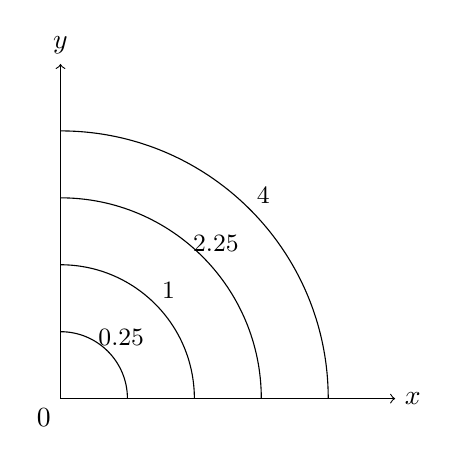
\begin{tikzpicture}[scale=1.7]
      \draw[->] (0,0) -- (2.5,0) node[right] {$x$};
      \draw[->] (0,0) -- (0,2.5) node[above] {$y$};

      \foreach \r/\label in {0.5/0.25, 1/1, 1.5/2.25, 2/4} {
        \draw (0,\r) arc[start angle=90, end angle=0, radius=\r];
        \node at ({\r/sqrt(2) + 0.1}, {\r/sqrt(2) + 0.1}) {\small $\label$};
      }

      \node[below left] at (0,0) {$0$};
    \end{tikzpicture}
    \end{center}
\end{itemize}
\begin{proposition}
  The gradient of $f$, $\nabla f$, is always normal to a level surface.
\end{proposition}
\begin{proof}
  Starting at a point $\vec{x}$ on the level surface, consider a small displacement $\d{\vec{x}}$ such that $\vec{x} + \d{\vec{x}}$ still lies on the surface.
  Since $f = c$ on the surface, $\d{f} = 0$ for this displacement.
  Using \cref{infinitesimalsGrad}, we have:
  \[
    \d{f} = \nabla f \cdot \d{\vec{x}} = 0
  \]
  Therefore, $\nabla f$ is perpendicular to $\d{\vec{x}}$ for all possible choices of $\d{\vec{x}}$, that is, it is normal to the level surface.
\end{proof}
\begin{example}
  In \cref{gradExample}, we saw that if $f(\vec{x}) = |\vec{x}|^2$, then $\nabla f = 2\vec{x}$.
  $f(\vec{x}) = c \implies |\vec{x}| = r$ so the level surfaces of $f$ are just spheres centered at the origin.
  We also see that $\nabla f$ points radially outwards, which is normal to each sphere, as expected.
\end{example}
Since $D_{\vec{n}} f = \vec{n} \cdot \nabla f$ for any unit vector $\vec{n}$:
\begin{itemize}
  \item $D_{\vec{n}}$ is maximised when $\vec{n}$ points in the same direction to $\nabla f$.
  \item $D_{\vec{n}} = 0$ when $\vec{n}$ is orthogonal to $\nabla f$ (i.e. $\vec{n}$ is tangent to the level surface).
  \item $D_{\vec{n}}$ is minimised when $\vec{n}$ points in the opposite direction to $\nabla f$.
\end{itemize}
\[
  \max_{\forall \vec{n}} D_{\vec{n}} = |\nabla f| \text{ and } \min_{\forall \vec{n}} D_{\vec{n}} = -|\nabla f|
\]
Furthermore, since $\nabla f$ is normal to the level surfaces, the directional derivative is maximised along the normals of the surface that point in the direction of increasing $f$.

\begin{remark}[Defining level sufaces in two ways]
  We can think of level surfaces in two ways.

  Suppose the ground height is defined by $z = h(x, y)$ where $z$ is the height about some fixed level.
  We can think of this in terms of the 2D function $h$, or by defining the 3D function $f(x, y, z) = z - h(x, y)$ and then considering the level surface $f = 0$.

  In terms of $h$, $\nabla h \in \R^2$ points in the direction that is steepest uphill on the surface and then projected down onto the $x$-$y$ plane.
  However, if we use $f = 0$, which defines exactly the same surface, then $\nabla f$ instead points normal to the surface as it is a level surface, so we need to be careful about our interpretations of grad depending on how we define the surface.

  Note that the choice of $f$ here is by no means unique.
  For example, defining $g(\vec{x}) = h^3 + 1 - z^3$ and considering the level surface $g = 1$ defines exactly the same surface.
\end{remark}
\section{Vector Differential Identities}
For scalar fields $f, g$ and vector fields $\vec{F}, \vec{G}$, we have the following identities for grad, div, and curl:
\begin{align*}
  \nabla(fg) &= f \nabla g + g \nabla f  \\
  \nabla[f(g(\vec{x}))] &= f'(g(\vec{x})) \nabla g \\
  \nabla \cdot (f\vec{F}) &= f (\nabla \cdot \vec{F}) + \vec{F} \cdot (\nabla f) \tag{$\dag$} \label{gradDotfF} \\
  \nabla \times (f\vec{F}) &= f (\nabla \times \vec{F}) + (\nabla f) \times \vec{F} \\
  \nabla (\vec{F} \cdot \vec{G}) &= \vec{F} \times (\nabla \times \vec{G}) + (\vec{F} \cdot \nabla)\vec{G} + \vec{G} \times (\nabla \times \vec{F}) + (\vec{G} \cdot \nabla)\vec{F} \tag{$\star$} \label{gradFG} \\
  \nabla \cdot (\vec{F} \times \vec{G}) &= - \vec{F} \cdot (\nabla \times \vec{G}) + \vec{G} \cdot (\nabla \times \vec{F}) \\
  \nabla \times (\vec{F} \times \vec{G}) &= (\nabla \cdot \vec{G})\vec{F} - (\nabla \cdot \vec{F})\vec{G} + (\vec{G} \cdot \nabla)\vec{F} - (\vec{F} \cdot \nabla) \vec{G}
\end{align*}
These can all be proved with suffix notation.
For example:
\begin{proof}[For \cref{gradDotfF}]
  \begin{align*}
    \nabla \cdot (f \vec{F}) &= \pderiv{}{x_i}(fF_i) \\
                             &= \pderiv{f}{x_i} F_i + f \pderiv{F_i}{x_i} \\
                             &= \vec{F} \cdot (\nabla f) + f \nabla \cdot \vec{F}
  \end{align*}
\end{proof}
\begin{proof}[For \cref{gradFG}]
  Working from the right hand side:
  \begin{align*}
    (\vec{F} \times (\nabla \times \vec{G}))_i &= \levi_{i j k} F_j \levi_{k l m} \pderiv{}{x_l}G_m \\
                                               &= (\delta_{i l}\delta_{j m} - \delta_{i m}\delta_{j l}) F_j \pderiv{G_m}{x_l} \\
                                               &= F_j \pderiv{G_j}{x_i} - F_j \pderiv{G_i}{x_j}
  \end{align*}
  and similarly $(G \times (\nabla \times \vec{F}))_i = G_j \pderiv{F_j}{x_i} - G_j \pderiv{F_i}{x_j}$.

  So:
  \begin{align*}
    (\vec{F} \times (\nabla \times \vec{G}) + \vec{G} \times (\nabla \times \vec{F}))_i &= F_j \pderiv{G_j}{x_i} - F_j \pderiv{G_i}{x_j} + G_j \pderiv{F_j}{x_i} - G_j \pderiv{F_i}{x_j} \\
                                                                                        &= \left(F_j \pderiv{G_j}{x_i} + G_j \pderiv{F_j}{x_i}\right) - \left(F_j \pderiv{G_i}{x_j} + G_j \pderiv{F_i}{x_j}\right) \\
                                                                                        &= \pderiv{}{x_i}(F_jG_j) - ((\vec{F} \cdot \nabla)\vec{G})_i - ((\vec{G} \cdot \nabla)\vec{F})_i \\
                                                                                        &= \pderiv{}{x_i}(\vec{F} \cdot \vec{G}) - ((\vec{F} \cdot \nabla)\vec{G})_i - ((\vec{G} \cdot \nabla)\vec{F})_i
  \end{align*}
  Rearranging, we have:
  \[
    (\nabla(\vec{F} \cdot \vec{G}))_i = (\vec{F} \times (\nabla \times \vec{G}) + \vec{G} \times (\nabla \times \vec{F}))_i + ((\vec{F} \cdot \nabla)\vec{G})_i + ((\vec{G} \cdot \nabla)\vec{F})_i
  \]
  and so the result follows.
\end{proof}
\begin{remark}[Warning]
  The scalar triple product formula $\vec{a} \cdot (\vec{b} \times \vec{c}) = (\vec{a} \times \vec{b}) \cdot \vec{c}$ and the vector triple product formula $\vec{a} \times (\vec{b} \times \vec{c}) = (\vec{a} \cdot \vec{c}) \vec{b} - (\vec{a} \cdot \vec{b}) \vec{c}$ do not work if one of the vectors is $\nabla$.
  This is because the proofs for these identities assume commutativity of the components of the vectors which is not true when the components are operators.

  For example, $\vec{a} \times (\nabla \times \vec{c}) \neq (\vec{a} \cdot \vec{c})\nabla - (\vec{a} \cdot \nabla)\vec{c}$ and this is both wrong and meaningless as $(\vec{a} \cdot \vec{c}) \nabla$ is an operator, not a vector.

  When proving these identities, you need to make sure that operators and functions stay in the same order.
\end{remark}
\begin{proposition}
  Another very useful identity is:
  \[
    \pderiv{r}{x_i} = \frac{x_i}{r}
  \]
\end{proposition}
\begin{proof}
  We defined $r = |\vec{x}|$ and know from \cref{gradExample} that $\nabla(|\vec{x}|) = \frac{\vec{x}}{|\vec{x}|}$ so:
  \[
    \pderiv{r}{x_i} = [\nabla(r)]_i = \left[\frac{\vec{x}}{r}\right]_i = \frac{x_i}{r}
  \]
\end{proof}
\begin{corollary}
  \[
    \nabla f(r) = f'(r)\vec{e}_r \text{ where } \vec{e}_r = \frac{\vec{x}}{r}
  \]
\end{corollary}
\begin{proof}
  \[
    (\nabla f(r))_i = \pderiv{}{x_i}f(r) = f'(r) \pderiv{r}{x_i} = f'(r) \frac{x_i}{r}
  \]
  So $\nabla f(r) = \frac{\vec{x}}{r} = \vec{e}_r$ which is a unit vector in the radial direction of $\vec{x}$.
\end{proof}
\section{Laplacian}
\label{secLaplacian}
\section{Summary}
Here is a summary of the various vector differential operators and their actions on a scalar field $f$ and vector field $\vec{F}$:
\begin{center}
\begin{tabular}{c||c|c|c|c}
  \textbf{Operator} & \textbf{Symbol} &  \textbf{Result on} $f$ & \textbf{Result on} $\vec{F}$ & \textbf{Reference} \\
\hline
  Grad & $\nabla$ & Vector & -- & \Cref{secGrad} \\
  Divergence & $\nabla \cdot $ & -- & Scalar & \Cref{secDiv} \\
  Curl & $\nabla \times $ & -- & Vector & \Cref{secCurl} \\
  $u$ dot del & $\vec{u} \cdot \nabla$ & Scalar & Vector & \Cref{secUdot} \\
  Laplacian & $\nabla^2$ & Scalar & Vector & \Cref{secLaplacian} \\
\end{tabular}
\end{center}
\end{document}
